\documentclass[12pt,a4paper]{article}
    \usepackage{graphicx}
    \usepackage[french]{babel}
    \usepackage[utf8]{inputenc}
    \usepackage{tikz}
    \usepackage{amsfonts}
    \usepackage{float}
    \usetikzlibrary {positioning}
    
    \begin{document}
    \begin{titlepage}
        \centering
        {\scshape\LARGE ENSIMAG - Grenoble INP \par}
        \vspace{1cm}
        {\scshape\Large 3MM1PA - Probabilités Appliquées\par}
        \vspace{1.5cm}
        {\huge\bfseries Simulation d'une file d'attente\par}
        \vspace{2cm}
        {\Large Othmane AJDOR\par}
        \vfill
        encadré par\par
        Dr.~Hervé \textsc{Guiol}
    
        \vfill
    
    
        {\large \today\par}
    \end{titlepage}
    
    \tableofcontents
    
    % Sujet
    %\newpage
    %    \section*{Sujet}
    %    \paragraph{}
    %    Simuler une file d'attente sur un serveur:
    %    \begin{itemize}
    %        \item Un serveur reçoit une requête suivant une %intensité $\lambda > 1$
    %        \item Le temps moyen de traitement d'une requête est %$\frac{1}{\mu}$ où $\mu > 0$
    %        \item Le serveur a une capacité maximale de stockage %des requêtes de \linebreak $N \in \mathbb{N}$. 
    %         Au delà, la requête est perdue.
    %        \item On a le choix sur l'ordre de priorité de %traitement des requêtes.
    %        \item On suppose qu'on a 3 types de requêtes:
    %            \begin{enumerate}
    %                \item Prioritaire
    %                \item Normale
    %                \item Lente
    %            \end{enumerate}
    %        \item la proportion de prioritaire est $p_1$, normale %$p_2$ et lente $p_3$.
    %    \end{itemize}
    %
    %    \paragraph{}
    %    Questions:
    %    \begin{itemize}
    %        \item Quel système garanti au mieux le traitement en %tenant compte des priorités.
    %        \item Quelle est la probabilité de perte.
    %        \item Combien de serveur faudrait-il rajouter pour %garantir un bon traitement.
    %    \end{itemize}
        
    % End sujet
    
    % Graph
    \newpage{}
    \section{File d'attente}
        
        \subsection{Arrivée des requêtes}

        \par Dans cette simulation, les requêtes arrivent à des instants aléatoires $T_1$, $T_2$, ..., $T_n$ suivant une loi exponentielle $exp(\lambda)$.\newline
        Sachant que le serveur ne peut accepter qu'une requête par instant dans la file d'attente, celle-ci est rangée dans une sous-file d'attente selon son type en incrémentant le nombre de requêtes dans la file d'attente.
        Soit prioritaire, normale ou lente avec des proportions $p_1$, $p_2$ et $p_3$ respectivement.\newline
        L'ordre de priorité de cette requête est décidé selon une variable aléatoire $0\leq p\leq 1$.
        Cela peut être représenté sur un graph par des transitions entre états: 
        
        \begin{figure}[H]
            \begin {center}
            \begin {tikzpicture}[-latex ,auto ,node distance =1 cm and 2.4cm ,on grid ,
            state/.style ={ circle ,top color =white , draw, minimum width =1.5 cm}]
            \node[state] (A) {$0$};
            \node[state] (B) [right=of A] {$1$};
            \node[state] (C) [right=of B] {$2$};
            \node[state] (D) [right=of C] {$...$};
            \node[state] (E) [right=of D] {$N-1$};
            \node[state] (F) [right=of E] {$N$};
            %\path (A) edge [loop above] node[left] {$\lambda$} (A);
            \path (A) edge [bend left =50] node[above =0.15 cm] {$\lambda$} (B);
            \path (B) edge [bend left =50] node[above =0.15 cm] {$\lambda$} (C);
            \path (C) edge [bend left =50] node[above =0.15 cm] {$\lambda$} (D);
            \path (D) edge [bend left =50] node[above =0.15 cm] {$\lambda$} (E);
            \path (E) edge [bend left =50] node[above =0.15 cm] {$\lambda$} (F);
            \end{tikzpicture}
            \end{center}
            \caption{Arrivée des requêtes}
        \end{figure}
        
        \subsection{Traitement et départ des requêtes}

        \par
        Ces requêtes sont traitées à des instants aléatoires $S_1$, $S_2$, ..., $S_n$ suivant une loi exponentielle $exp(\mu)$.\newline
        Les requêtes sont traitées dans l'ordre de priorité précédemment défini. Tant qu'il reste des requêtes prioritaires dans la file d'attente, celles-ci sont traitées avant de passer aux normales puis aux requêtes lentes.\newline
        Le graph alors devient:
        
        \begin{figure}[H]
            \begin {center}
            \begin {tikzpicture}[-latex ,auto ,node distance =1 cm and 2.4cm ,on grid ,
            state/.style ={ circle ,top color =white , draw, minimum width =1.5 cm}]
            \node[state] (A) {$0$};
            \node[state] (B) [right=of A] {$1$};
            \node[state] (C) [right=of B] {$2$};
            \node[state] (D) [right=of C] {$...$};
            \node[state] (E) [right=of D] {$N-1$};
            \node[state] (F) [right=of E] {$N$};
            %\path (A) edge [loop above] node[left] {$\lambda$} (A);
            \path (A) edge [bend left =50] node[above =0.15 cm] {$\lambda$} (B);
            \path (B) edge [bend left =50] node[below =0.15 cm] {$\mu$} (A);
            \path (B) edge [bend left =50] node[above =0.15 cm] {$\lambda$} (C);
            \path (C) edge [bend left =50] node[below =0.15 cm] {$\mu$} (B);
            \path (C) edge [bend left =50] node[above =0.15 cm] {$\lambda$} (D);
            \path (D) edge [bend left =50] node[below =0.15 cm] {$\mu$} (C);
            \path (D) edge [bend left =50] node[above =0.15 cm] {$\lambda$} (E);
            \path (E) edge [bend left =50] node[below =0.15 cm] {$\mu$} (D);
            \path (E) edge [bend left =50] node[above =0.15 cm] {$\lambda$} (F);
            \path (F) edge [bend left =50] node[below =0.15 cm] {$\mu$} (E);
            \end{tikzpicture}
            \end{center}
            \caption{Arrivée et traitement des requêtes}
        \end{figure}
        
        
    \newpage
    \section{Multi-serveur}
    \par La simulation permet de personnaliser le nombre de serveur traitant les requêtes dans la file d'attente.\newline
    En augmentant le nombre de serveur, le nombre de requêtes traitées par cycle augmente tant qu'il y a une correspondance entre les deux nombres. Si le nombre de requêtes est moins important, ajouter des serveurs supplémentaires pour accélérer le traitement implique un temps Idle conséquent. Les serveurs passent alors la plupart du temps en mode Standby attendant de nouvelles requêtes.
    \newline\par
    Inversement, si le nombre de requêtes dans la file est assez grand, alors que le nombre de serveur ainsi que la taille de la file d'attente sont limités, des requêtes ne sont pas traitées et sont par conséquent perdues.
    \newline
    La génération d'un temps de traitement dans le mode multi-serveur repose sur la décision du temps le plus éloigné de l'instant courant.
    \newline
    
    \begin{figure}[H]
        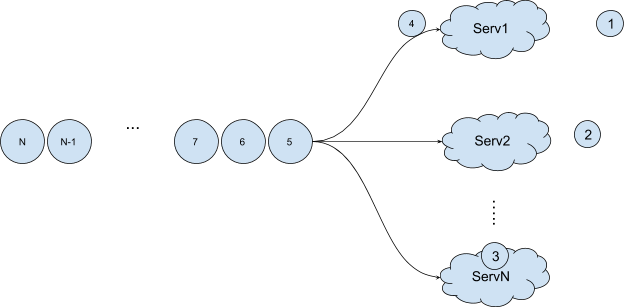
\includegraphics[scale=0.6]{servers.png}
        \caption{Traitement des requêtes par N serveurs}
    \end{figure}
    
        \newpage
    \section{Résultats}
    Dans la suite des simulation suivante, on considère le temps de simulation $duration = 10^4$, la capacité de la file d'attente $N = 150$, la proportion des requêtes prioritaires $fP = 0.1$ et la proportion des requêtes normales $nP = 0.3$.
    \subsection{Perte de requête}
    \par Dans la simulation suivante, on considère que le nombre de serveurs traitant les requêtes $nS = 1$ pour un paramètre $\lambda = [{0.1},{10}]$ et $ \mu = 1$.
    
    \begin{center}
        \begin{figure}[H]
            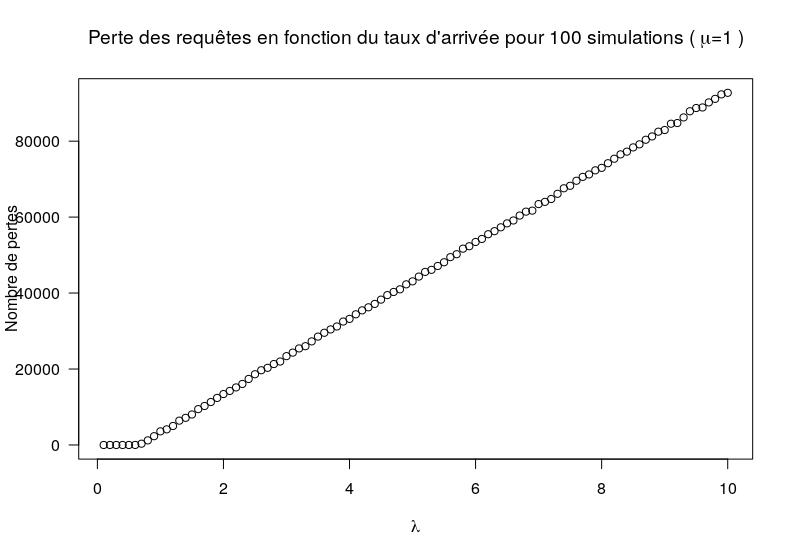
\includegraphics[scale=0.7]{lostQueries.png}
            \caption{Traitement des requêtes par N serveurs}
        \end{figure}
    \end{center}
    
    On observe dans le résultat de cette simulation que le nombre de requêtes perdues augmente de façon linéaire à partir de $\lambda = 0.7$ et dépasse les 80000 requêtes perdues à partir de $\lambda = 9$ par rapport à $\mu = 1$.
    
    \subsection{Taux d'utilisation multi-serveur}
    \par Dans la simulation suivante, on considère que $\lambda = 2$, $\mu = 1$ et un paramètre $nS = [{1},{50}]$.
    
    \begin{center}
        \begin{figure}[H]
            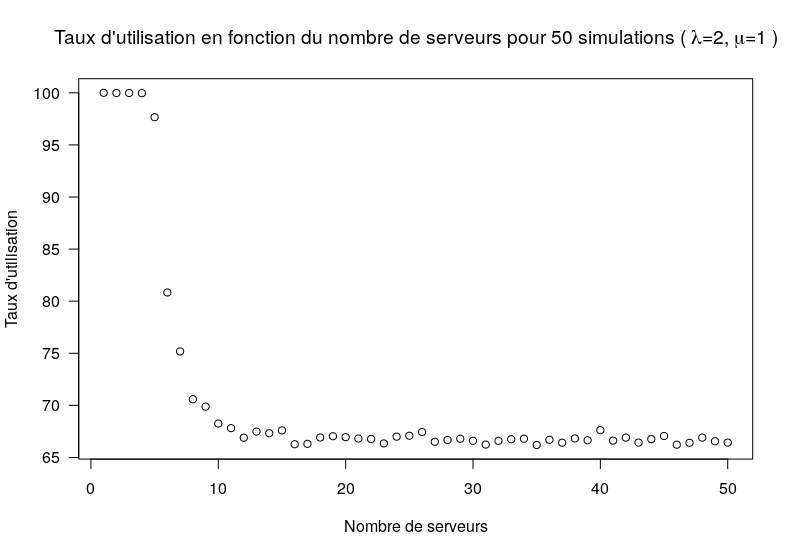
\includegraphics[scale=0.7]{busyRate.png}
            \caption{Traitement des requêtes par N serveurs}
        \end{figure}
    \end{center}

    On observe dans le résultat de cette simulation que le taux d'utilisation est constant à environ $100\%$ pour $nS = [{1},{4}]$ et commence à diminuer jusqu'à atteindre une valeur comprise entre 65 et 70 pour $nS = [{9},{11}]$.
    \newline
    \par A partir de $nS = 10$, le taux d'utilisation se stabilise, ce qui signifie qu'augmenter le nombre de serveurs au delà de 10 ne contribue pas à la diminution de celui-ci.

    \newpage
    \subsection{Distribution des requêtes dans la file d'attente}
    \par Dans la simulation suivante, on considère que $\lambda = 1$, $\mu = 1$ et le nombre de serveurs $nS = 2$. On rappelle que la proportion des requêtes prioritaires est de 10\%, celle des requêtes normales 30\% et le reste est utilisé par les requêtes lentes. \newline
    On lance la simulation pour une durée de 100 instants pour une meilleure visibilité de la répartition des requêtes.
    
    \begin{center}
        \begin{figure}[H]
            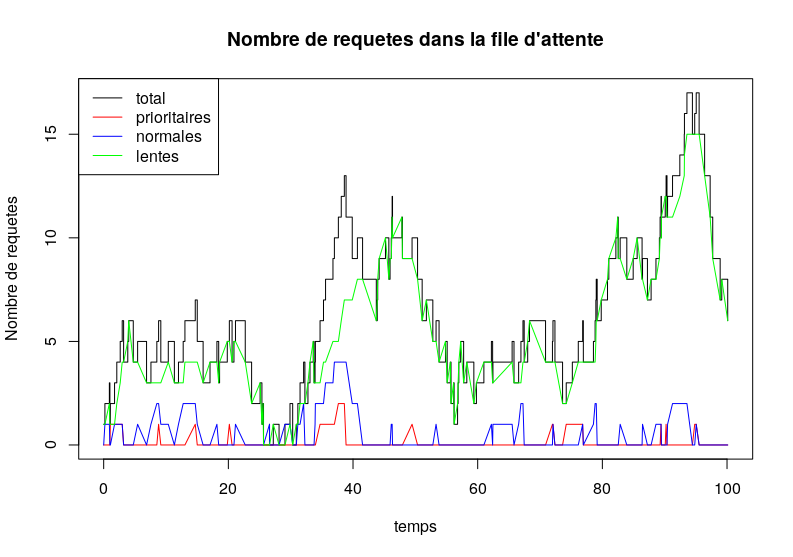
\includegraphics[scale=0.7]{queryDistribution.png}
            \caption{Distribution des requêtes durant les 100 premiers instants}
        \end{figure}
    \end{center}

    On observe dans le résultat de cette simulation que le nombre de requêtes varie bien en fonction de la proportion des requêtes dans la file d'attente. Soit le nombre de requêtes prioritaire $\leq 2$, celui des requêtes normales $\leq 5$, et le reste est occupé par les requêtes lentes dont la proportion est la plus importante.


    
\end{document}
    
    